\documentclass[border=10pt]{standalone}

\usepackage{tikz}
\usepackage{tikzsymbols}
\usetikzlibrary{calc,patterns,shapes.geometric}

\def\centerarc[#1](#2)(#3:#4:#5){\draw[#1] ($(#2)+({#5*cos(#3)},{#5*sin(#3)})$) arc (#3:#4:#5);}

\begin{document}
	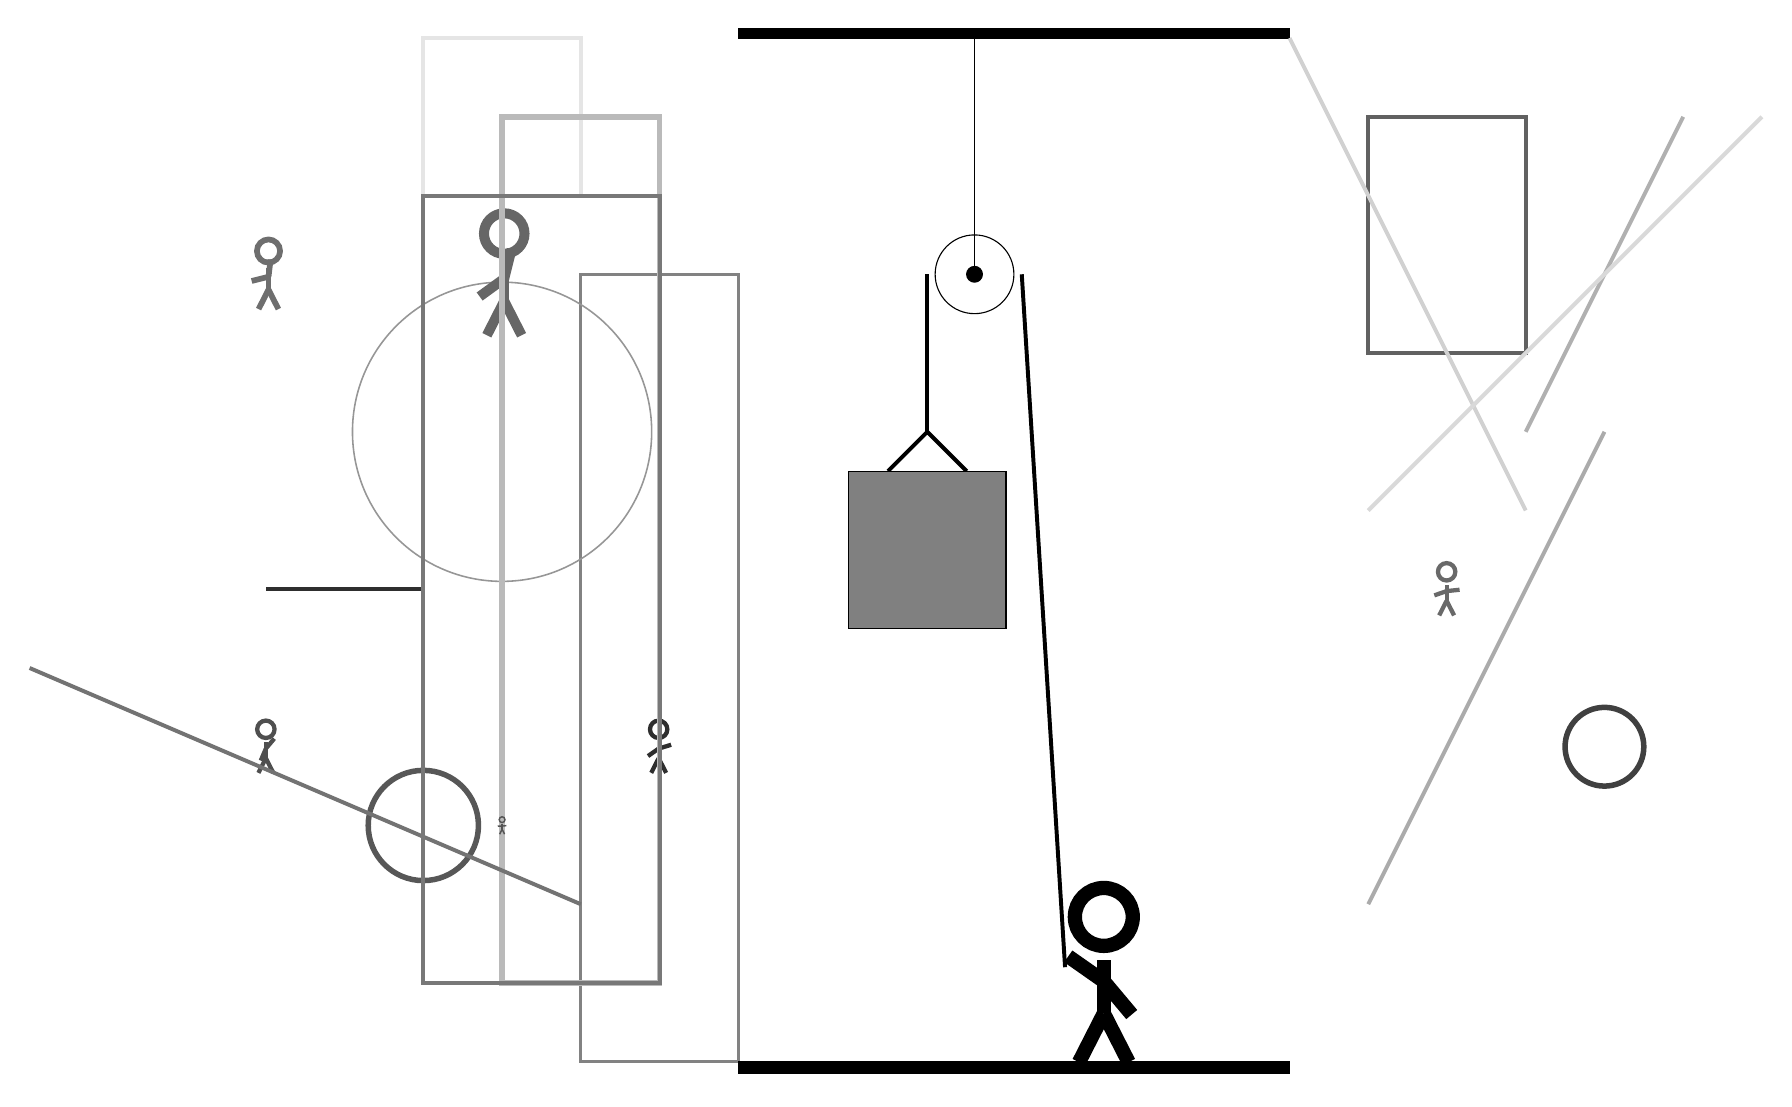
\begin{tikzpicture}
		%%%%% START %%%%%
		
		\draw[fill=black] (-2, 10) rectangle (5, 10.125);
		
		\draw[line width=0.5mm, color=black!82](-6, 3) -- (-8, 3);
		
		\draw[line width=0.5mm, color=black!31](10, 9) -- (8, 5);
		\draw[line width=0.4mm, color=black!49] (-2, 7) rectangle (-4, -3);
		\node[line width=0.6mm, color=black!69] at (-8, 1) {\Strichmaxerl[3][67][50]};
		\draw[line width=0.5mm, color=black!33](6, -1) -- (9, 5);
		\draw [line width=0.7mm, color=black!75](9, 1) circle (0.5);
		\draw [line width=0.7mm, color=black!66](-6, 0) circle (0.7);
		
		\draw [line width=0.2mm, color=black!41](-5, 5) circle (1.9);
		\node[line width=0.4mm, color=black!60] at (-5, 7) {\Strichmaxerl[7][36][76]};
		
		\node[line width=0.5mm, color=black!82] at (-3, 1) {\Strichmaxerl[3][35][17]};
		\draw[line width=0.5mm, color=black!62] (6, 9) rectangle (8, 6);
		
		\draw[line width=0.5mm, color=black!10] (-4, 8) rectangle (-6, 10);
		\draw[line width=0.7mm, color=black!27] (-3, 9) rectangle (-5, -2);
		\node[line width=0.6mm, color=black!67] at (-5, 0) {\Strichmaxerl[1][1][6]};
		\draw[line width=0.5mm, color=black!55](-4, -1) -- (-11, 2);
		\draw[line width=0.5mm, color=black!53] (-3, 8) rectangle (-6, -2);
		
		\node[line width=0.5mm, color=black!57] at (-8, 7) {\Strichmaxerl[4][14][83]};
		\draw[line width=0.5mm, color=black!18](8, 4) -- (5, 10);
		\draw[line width=0.5mm, color=black!15](6, 4) -- (11, 9);
		\node[line width=0.7mm, color=black!59] at (7, 3) {\Strichmaxerl[3][19][6]};
		
		\draw (1, 7) circle (0.5);
		\draw[fill=black] (1, 7) circle (0.1);
		\draw (1, 10) -- (1, 7);
		
		\draw[line width=0.5mm] (-0.1, 4.5) -- (0.4, 5.0) -- (0.9, 4.5);
		\draw[fill=black!50] (-0.6, 4.5) rectangle (1.4, 2.5);
		
		\draw[line width=0.5mm] (0.4, 7) -- (0.4, 5.0);
		\centerarc[line width=0.5mm](1, 7)(0:180:0.6);
		\draw[line width=0.5mm](1.6, 7) -- (2.15, -1.8);
		
		\node at (2.6, -1.9) {\Strichmaxerl[10][-35][-50]};
		
		\draw[fill=black] (-2, -3) rectangle (5, -3.15);
		
		%%%%% END %%%%%
	\end{tikzpicture}
\end{document}